% Options for packages loaded elsewhere
\PassOptionsToPackage{unicode}{hyperref}
\PassOptionsToPackage{hyphens}{url}
\PassOptionsToPackage{dvipsnames,svgnames,x11names}{xcolor}
%
\documentclass[
]{article}
\usepackage{amsmath,amssymb}
\usepackage{lmodern}
\usepackage{iftex}
\ifPDFTeX
  \usepackage[T1]{fontenc}
  \usepackage[utf8]{inputenc}
  \usepackage{textcomp} % provide euro and other symbols
\else % if luatex or xetex
  \usepackage{unicode-math}
  \defaultfontfeatures{Scale=MatchLowercase}
  \defaultfontfeatures[\rmfamily]{Ligatures=TeX,Scale=1}
\fi
% Use upquote if available, for straight quotes in verbatim environments
\IfFileExists{upquote.sty}{\usepackage{upquote}}{}
\IfFileExists{microtype.sty}{% use microtype if available
  \usepackage[]{microtype}
  \UseMicrotypeSet[protrusion]{basicmath} % disable protrusion for tt fonts
}{}
\makeatletter
\@ifundefined{KOMAClassName}{% if non-KOMA class
  \IfFileExists{parskip.sty}{%
    \usepackage{parskip}
  }{% else
    \setlength{\parindent}{0pt}
    \setlength{\parskip}{6pt plus 2pt minus 1pt}}
}{% if KOMA class
  \KOMAoptions{parskip=half}}
\makeatother
\usepackage{xcolor}
\usepackage{graphicx}
\makeatletter
\def\maxwidth{\ifdim\Gin@nat@width>\linewidth\linewidth\else\Gin@nat@width\fi}
\def\maxheight{\ifdim\Gin@nat@height>\textheight\textheight\else\Gin@nat@height\fi}
\makeatother
% Scale images if necessary, so that they will not overflow the page
% margins by default, and it is still possible to overwrite the defaults
% using explicit options in \includegraphics[width, height, ...]{}
\setkeys{Gin}{width=\maxwidth,height=\maxheight,keepaspectratio}
% Set default figure placement to htbp
\makeatletter
\def\fps@figure{htbp}
\makeatother
\setlength{\emergencystretch}{3em} % prevent overfull lines
\providecommand{\tightlist}{%
  \setlength{\itemsep}{0pt}\setlength{\parskip}{0pt}}
\setcounter{secnumdepth}{-\maxdimen} % remove section numbering
% definitions for citeproc citations
\NewDocumentCommand\citeproctext{}{}
\NewDocumentCommand\citeproc{mm}{%
  \begingroup\def\citeproctext{#2}\cite{#1}\endgroup}
\makeatletter
 % allow citations to break across lines
 \let\@cite@ofmt\@firstofone
 % avoid brackets around text for \cite:
 \def\@biblabel#1{}
 \def\@cite#1#2{{#1\if@tempswa , #2\fi}}
\makeatother
\newlength{\cslhangindent}
\setlength{\cslhangindent}{1.5em}
\newlength{\csllabelwidth}
\setlength{\csllabelwidth}{3em}
\newenvironment{CSLReferences}[2] % #1 hanging-indent, #2 entry-spacing
 {\begin{list}{}{%
  \setlength{\itemindent}{0pt}
  \setlength{\leftmargin}{0pt}
  \setlength{\parsep}{0pt}
  % turn on hanging indent if param 1 is 1
  \ifodd #1
   \setlength{\leftmargin}{\cslhangindent}
   \setlength{\itemindent}{-1\cslhangindent}
  \fi
  % set entry spacing
  \setlength{\itemsep}{#2\baselineskip}}}
 {\end{list}}
\usepackage{calc}
\newcommand{\CSLBlock}[1]{\hfill\break\parbox[t]{\linewidth}{\strut\ignorespaces#1\strut}}
\newcommand{\CSLLeftMargin}[1]{\parbox[t]{\csllabelwidth}{\strut#1\strut}}
\newcommand{\CSLRightInline}[1]{\parbox[t]{\linewidth - \csllabelwidth}{\strut#1\strut}}
\newcommand{\CSLIndent}[1]{\hspace{\cslhangindent}#1}
\ifLuaTeX
\usepackage[bidi=basic]{babel}
\else
\usepackage[bidi=default]{babel}
\fi
\babelprovide[main,import]{american}
% get rid of language-specific shorthands (see #6817):
\let\LanguageShortHands\languageshorthands
\def\languageshorthands#1{}
\ifLuaTeX
  \usepackage{selnolig}  % disable illegal ligatures
\fi
\IfFileExists{bookmark.sty}{\usepackage{bookmark}}{\usepackage{hyperref}}
\IfFileExists{xurl.sty}{\usepackage{xurl}}{} % add URL line breaks if available
\urlstyle{same} % disable monospaced font for URLs
\hypersetup{
  pdftitle={SlicerNNInteractive: A 3D Slicer extension for
nnInteractive},
  pdfauthor={Coen de Vente, Kiran Vaidhya Venkadesh, Andras Lasso, Bram
van Ginneken, Clara I. Sánchez},
  pdflang={en-US},
  colorlinks=true,
  linkcolor={Maroon},
  filecolor={Maroon},
  citecolor={Blue},
  urlcolor={Blue},
  pdfcreator={LaTeX via pandoc}}

\title{SlicerNNInteractive: A 3D Slicer extension for nnInteractive}

\definecolor{c53baa1}{RGB}{83,186,161}
\definecolor{c202826}{RGB}{32,40,38}
\def \rorglobalscale {0.1}
\newcommand{\rorlogo}{%
\begin{tikzpicture}[y=1cm, x=1cm, yscale=\rorglobalscale,xscale=\rorglobalscale, every node/.append style={scale=\rorglobalscale}, inner sep=0pt, outer sep=0pt]
  \begin{scope}[even odd rule,line join=round,miter limit=2.0,shift={(-0.025, 0.0216)}]
    \path[fill=c53baa1,nonzero rule,line join=round,miter limit=2.0] (1.8164, 3.012) -- (1.4954, 2.5204) -- (1.1742, 3.012) -- (1.8164, 3.012) -- cycle;
    \path[fill=c53baa1,nonzero rule,line join=round,miter limit=2.0] (3.1594, 3.012) -- (2.8385, 2.5204) -- (2.5172, 3.012) -- (3.1594, 3.012) -- cycle;
    \path[fill=c53baa1,nonzero rule,line join=round,miter limit=2.0] (1.1742, 0.0669) -- (1.4954, 0.5588) -- (1.8164, 0.0669) -- (1.1742, 0.0669) -- cycle;
    \path[fill=c53baa1,nonzero rule,line join=round,miter limit=2.0] (2.5172, 0.0669) -- (2.8385, 0.5588) -- (3.1594, 0.0669) -- (2.5172, 0.0669) -- cycle;
    \path[fill=c202826,nonzero rule,line join=round,miter limit=2.0] (3.8505, 1.4364).. controls (3.9643, 1.4576) and (4.0508, 1.5081) .. (4.1098, 1.5878).. controls (4.169, 1.6674) and (4.1984, 1.7642) .. (4.1984, 1.8777).. controls (4.1984, 1.9719) and (4.182, 2.0503) .. (4.1495, 2.1132).. controls (4.1169, 2.1762) and (4.0727, 2.2262) .. (4.0174, 2.2635).. controls (3.9621, 2.3006) and (3.8976, 2.3273) .. (3.824, 2.3432).. controls (3.7505, 2.359) and (3.6727, 2.367) .. (3.5909, 2.367) -- (2.9676, 2.367) -- (2.9676, 1.8688).. controls (2.9625, 1.8833) and (2.9572, 1.8976) .. (2.9514, 1.9119).. controls (2.9083, 2.0164) and (2.848, 2.1056) .. (2.7705, 2.1791).. controls (2.6929, 2.2527) and (2.6014, 2.3093) .. (2.495, 2.3487).. controls (2.3889, 2.3881) and (2.2728, 2.408) .. (2.1468, 2.408).. controls (2.0209, 2.408) and (1.905, 2.3881) .. (1.7986, 2.3487).. controls (1.6925, 2.3093) and (1.6007, 2.2527) .. (1.5232, 2.1791).. controls (1.4539, 2.1132) and (1.3983, 2.0346) .. (1.3565, 1.9436).. controls (1.3504, 2.009) and (1.3351, 2.0656) .. (1.3105, 2.1132).. controls (1.2779, 2.1762) and (1.2338, 2.2262) .. (1.1785, 2.2635).. controls (1.1232, 2.3006) and (1.0586, 2.3273) .. (0.985, 2.3432).. controls (0.9115, 2.359) and (0.8337, 2.367) .. (0.7519, 2.367) -- (0.1289, 2.367) -- (0.1289, 0.7562) -- (0.4837, 0.7562) -- (0.4837, 1.4002) -- (0.6588, 1.4002) -- (0.9956, 0.7562) -- (1.4211, 0.7562) -- (1.0118, 1.4364).. controls (1.1255, 1.4576) and (1.2121, 1.5081) .. (1.2711, 1.5878).. controls (1.2737, 1.5915) and (1.2761, 1.5954) .. (1.2787, 1.5991).. controls (1.2782, 1.5867) and (1.2779, 1.5743) .. (1.2779, 1.5616).. controls (1.2779, 1.4327) and (1.2996, 1.3158) .. (1.3428, 1.2113).. controls (1.3859, 1.1068) and (1.4462, 1.0176) .. (1.5237, 0.944).. controls (1.601, 0.8705) and (1.6928, 0.8139) .. (1.7992, 0.7744).. controls (1.9053, 0.735) and (2.0214, 0.7152) .. (2.1474, 0.7152).. controls (2.2733, 0.7152) and (2.3892, 0.735) .. (2.4956, 0.7744).. controls (2.6016, 0.8139) and (2.6935, 0.8705) .. (2.771, 0.944).. controls (2.8482, 1.0176) and (2.9086, 1.1068) .. (2.952, 1.2113).. controls (2.9578, 1.2253) and (2.9631, 1.2398) .. (2.9681, 1.2544) -- (2.9681, 0.7562) -- (3.3229, 0.7562) -- (3.3229, 1.4002) -- (3.4981, 1.4002) -- (3.8349, 0.7562) -- (4.2603, 0.7562) -- (3.8505, 1.4364) -- cycle(0.9628, 1.7777).. controls (0.9438, 1.7534) and (0.92, 1.7357) .. (0.8911, 1.7243).. controls (0.8623, 1.7129) and (0.83, 1.706) .. (0.7945, 1.7039).. controls (0.7588, 1.7015) and (0.7252, 1.7005) .. (0.6932, 1.7005) -- (0.4839, 1.7005) -- (0.4839, 2.0667) -- (0.716, 2.0667).. controls (0.7477, 2.0667) and (0.7805, 2.0643) .. (0.8139, 2.0598).. controls (0.8472, 2.0553) and (0.8768, 2.0466) .. (0.9025, 2.0336).. controls (0.9282, 2.0206) and (0.9496, 2.0021) .. (0.9663, 1.9778).. controls (0.9829, 1.9534) and (0.9914, 1.9209) .. (0.9914, 1.8799).. controls (0.9914, 1.8362) and (0.9819, 1.8021) .. (0.9628, 1.7777) -- cycle(2.6125, 1.3533).. controls (2.5889, 1.2904) and (2.5553, 1.2359) .. (2.5112, 1.1896).. controls (2.4672, 1.1433) and (2.4146, 1.1073) .. (2.3529, 1.0814).. controls (2.2916, 1.0554) and (2.2228, 1.0427) .. (2.1471, 1.0427).. controls (2.0712, 1.0427) and (2.0026, 1.0557) .. (1.9412, 1.0814).. controls (1.8799, 1.107) and (1.8272, 1.1433) .. (1.783, 1.1896).. controls (1.7391, 1.2359) and (1.7052, 1.2904) .. (1.6817, 1.3533).. controls (1.6581, 1.4163) and (1.6465, 1.4856) .. (1.6465, 1.5616).. controls (1.6465, 1.6359) and (1.6581, 1.705) .. (1.6817, 1.7687).. controls (1.7052, 1.8325) and (1.7388, 1.8873) .. (1.783, 1.9336).. controls (1.8269, 1.9799) and (1.8796, 2.0159) .. (1.9412, 2.0418).. controls (2.0026, 2.0675) and (2.0712, 2.0804) .. (2.1471, 2.0804).. controls (2.223, 2.0804) and (2.2916, 2.0675) .. (2.3529, 2.0418).. controls (2.4143, 2.0161) and (2.467, 1.9799) .. (2.5112, 1.9336).. controls (2.5551, 1.8873) and (2.5889, 1.8322) .. (2.6125, 1.7687).. controls (2.636, 1.705) and (2.6477, 1.6359) .. (2.6477, 1.5616).. controls (2.6477, 1.4856) and (2.636, 1.4163) .. (2.6125, 1.3533) -- cycle(3.8015, 1.7777).. controls (3.7825, 1.7534) and (3.7587, 1.7357) .. (3.7298, 1.7243).. controls (3.701, 1.7129) and (3.6687, 1.706) .. (3.6333, 1.7039).. controls (3.5975, 1.7015) and (3.5639, 1.7005) .. (3.5319, 1.7005) -- (3.3226, 1.7005) -- (3.3226, 2.0667) -- (3.5547, 2.0667).. controls (3.5864, 2.0667) and (3.6192, 2.0643) .. (3.6526, 2.0598).. controls (3.6859, 2.0553) and (3.7155, 2.0466) .. (3.7412, 2.0336).. controls (3.7669, 2.0206) and (3.7883, 2.0021) .. (3.805, 1.9778).. controls (3.8216, 1.9534) and (3.8301, 1.9209) .. (3.8301, 1.8799).. controls (3.8301, 1.8362) and (3.8206, 1.8021) .. (3.8015, 1.7777) -- cycle;
  \end{scope}
\end{tikzpicture}
}

%%%%%%%%%%%%%%%%%%%%%%%%%%%%%%%%%%%%%%%%%%%%%%%%%%%%%%%%%%%%%%%%%%%%%%%%
% Authors and Affiliations

\usepackage[affil-it]{authblk}
\usepackage{orcidlink}
%% \renewcommand\Authsep{, }
\setlength{\affilsep}{1em}
\author[1,2%
  %
  ]{Coen de Vente%
    \,\orcidlink{0000-0001-5908-8367}\,%
    }
\author[3%
  %
  ]{Kiran Vaidhya Venkadesh%
    \,\orcidlink{0000-0002-4846-9049}\,%
    }
\author[4%
  %
  ]{Andras Lasso%
    \,\orcidlink{0000-0002-4220-7064}\,%
    }
\author[3%
  %
  ]{Bram van Ginneken%
    \,\orcidlink{0000-0003-2028-8972}\,%
    }
\author[1,2%
  %
  ]{Clara I. Sánchez%
    \,\orcidlink{0000-0001-9787-8319}\,%
    }

\affil[1]{Quantitative Healthcare Analysis (qurAI) Group, Informatics
Institute, University of Amsterdam, Amsterdam, The Netherlands%
  }
\affil[2]{Amsterdam UMC location University of Amsterdam, Biomedical
Engineering and Physics, Amsterdam, The Netherlands%
  }
\affil[3]{Diagnostic Image Analysis Group (DIAG), Department of
Radiology and Nuclear Medicine, Radboud UMC, Nijmegen, The Netherlands%
  }
\affil[4]{Laboratory for Percutaneous Surgery, School of Computing,
Queen's University, Kingston, Canada%
  }
%%%%%%%%%%%%%%%%%%%%%%%%%%%%%%%%%%%%%%%%%%%%%%%%%%%%%%%%%%%%%%%%%%%%%%%%
\date{17 May 2025}

\begin{document}
\maketitle

\section{Summary}\label{summary}

\texttt{SlicerNNInteractive} integrates \texttt{nnInteractive}
(\citeproc{ref-isensee2025nninteractive}{Isensee et al., 2025}), a
state-of-the-art promptable deep learning-based framework for 3D image
segmentation, into the widely used \texttt{3D\ Slicer}
(\citeproc{ref-Kikinis2014}{Kikinis et al., 2014})
(\url{https://slicer.org}) platform. Our extension implements a
client-server architecture that decouples the computationally intensive
model inference from the client-side interface. Therefore,
\texttt{SlicerNNInteractive} eliminates heavy hardware constraints on
the client-side and enables better operating system compatibility than
existing plugins for \texttt{nnInteractive}. Running both the client and
server on a single machine is also possible, offering flexibility across
different deployment scenarios. The extension provides an intuitive user
interface with all interaction types available in the original framework
(point, bounding box, scribble, and lasso prompts), while including a
comprehensive set of keyboard shortcuts for efficient workflow.

\section{Statement of Need}\label{statement-of-need}

Segmentation is a cornerstone of medical image analysis. Manually
acquiring segmentation labels, however, is time-consuming and expensive.
Interactive segmentation tools can potentially accelerate this process
and reduce costs. Recently, \texttt{nnInteractive}
(\citeproc{ref-isensee2025nninteractive}{Isensee et al., 2025}), a deep
learning-based framework allowing for fast, promptable segmentation of
3D medical images was released and was shown to substantially outperform
existing approaches, such as SAM2
(\citeproc{ref-kirillov2023segment}{Kirillov et al., 2023}), SegVol
(\citeproc{ref-du2024segvol}{Du et al., 2024}), and SAM-Med-3D
(\citeproc{ref-wang2023sam}{Wang et al., 2023}). Alongside the
\texttt{nnInteractive} model, plugins in the medical image viewers MITK
(\citeproc{ref-MITK_Team_MITK_2024}{MITK~Team, 2024}) and Napari
(\citeproc{ref-Sofroniew2025-ty}{Sofroniew et al., 2025}) were
published. However, the original authors did not make an extension
available for \texttt{3D\ Slicer}, a widely used viewer and processing
environment in medical imaging research. Furthermore, these existing
plugins require substantial computational resources on the machine of
the image viewer itself (an NVIDIA GPU with at least 10 GB of VRAM is
recommended), as these plugins do not facilitate the deployment of the
backend on a separate server. Moreover, \texttt{nnInteractive} only runs
on Windows and Linux, so the image viewer cannot be run on MacOS
machines.

\texttt{SlicerNNInteractive} decouples the computationally intensive
\texttt{nnInteractive} inference by allowing users to configure a remote
server (e.g., a node of a GPU cluster), while running the client on a
machine with lower computational capabilities. This approach not only
broadens platform compatibility, but also addresses the resource
constraints of existing plugins, making \texttt{nnInteractive} more
widely available and potentially accelerating research related to
promptable segmentation.

\section{\texorpdfstring{Overview of
\texttt{SlicerNNInteractive}}{Overview of SlicerNNInteractive}}\label{overview-of-slicernninteractive}

\subsection{nnInteractive}\label{nninteractive}

While foundation models such as SAM (\citeproc{ref-ravi2024sam}{Ravi et
al., 2024}) and SAM2 (\citeproc{ref-kirillov2023segment}{Kirillov et
al., 2023}) have shown promising interactive segmentation performance in
2D natural images, their lack of volumetric awareness and the domain
shift from natural to medical data resulted in limited utility in 3D
medical imaging contexts. \texttt{nnInteractive} addresses these issues
through an nnUNet-based architecture
(\citeproc{ref-isensee2021nnu}{Isensee et al., 2021}) with residual
encoders (\citeproc{ref-isensee2024nnu}{Isensee et al., 2024}) that
supports diverse interation types: point, bounding box, scribble, and
lasso prompts. Trained on over 120 diverse volumetric datasets across
multiple modalities (CT, MRI, PET, 3D microscopy, etc.), the framework
demonstrated high accuracy and versatility. Our implementation extends
this capability to \texttt{3D\ Slicer}.

\subsection{Availability and
Installation}\label{availability-and-installation}

\texttt{SlicerNNInteractive} is available through multiple channels. The
server-side is available through Docker Hub
(\texttt{docker\ pull\ coendevente/nninteractive-slicer-server:latest}),
Pip (\texttt{pip\ install\ nninteractive-slicer-server}), and GitHub
(\url{https://github.com/coendevente/SlicerNNInteractive}). The
client-side is also available in the official \texttt{3D\ Slicer}
Extensions Manager.

\subsection{Client-server Setup}\label{client-server-setup}

\texttt{SlicerNNInteractive} uses a client-server setup, which decouples
the computationally intensive model inference from the
\texttt{3D\ Slicer} client. The server-side and client-side communicate
through FastAPI endpoints. An overview of the API is shown in
\autoref{fig:api_overview}. The client maintains synchronization between
the image and input segmentation in \texttt{3D\ Slicer}. To ensure a
smooth user experience, the client does not transfer this data each time
before processing a prompt, but only when this data have changed.

\begin{figure}
\centering
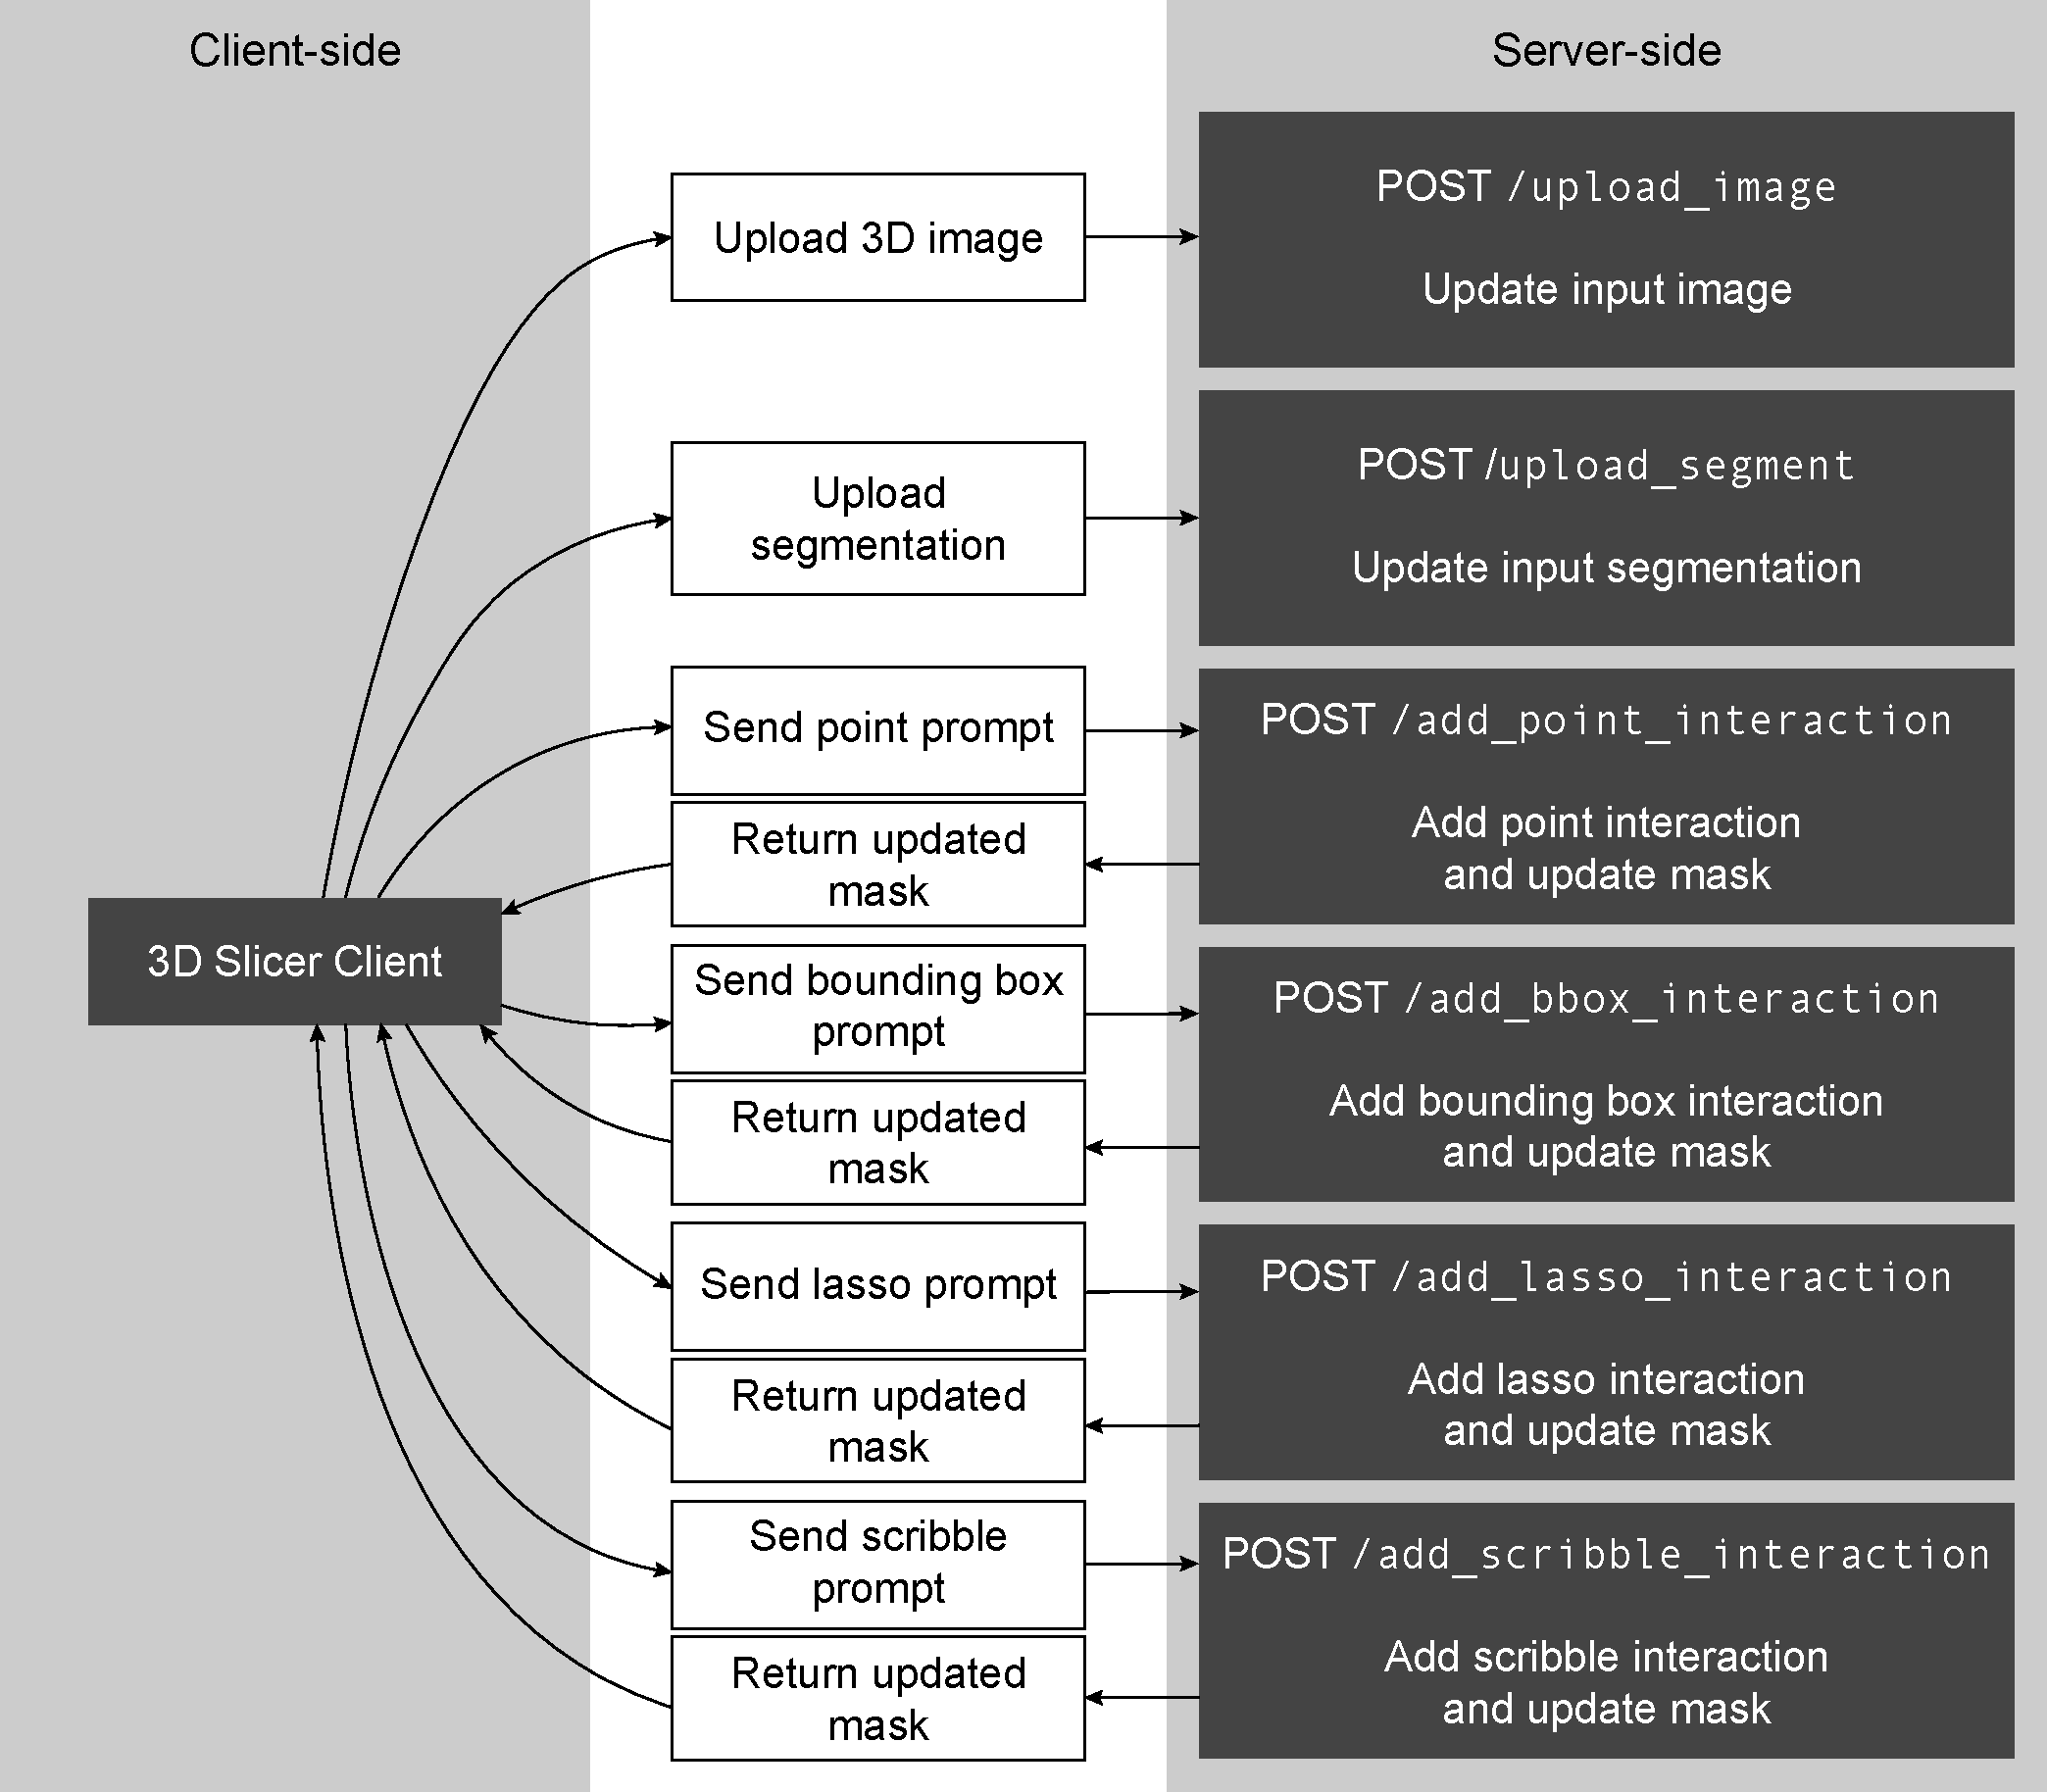
\includegraphics[width=0.8\textwidth,height=\textheight]{img/nni_api.pdf}
\caption{API overview.\label{fig:api_overview}}
\end{figure}

\subsection{User Interface}\label{user-interface}

The user interface of \texttt{SlicerNNInteractive} largely follows the
\texttt{nnInteractive} Napari and MITK plugins. A screenshot of the user
interface, including segmentation results, is shown in
\autoref{fig:screenshot}. A video showcasing the functionalities of the
extension is available
\href{https://www.youtube.com/watch?v=mW_fUT1-IWM}{here}.

\begin{figure}
\centering
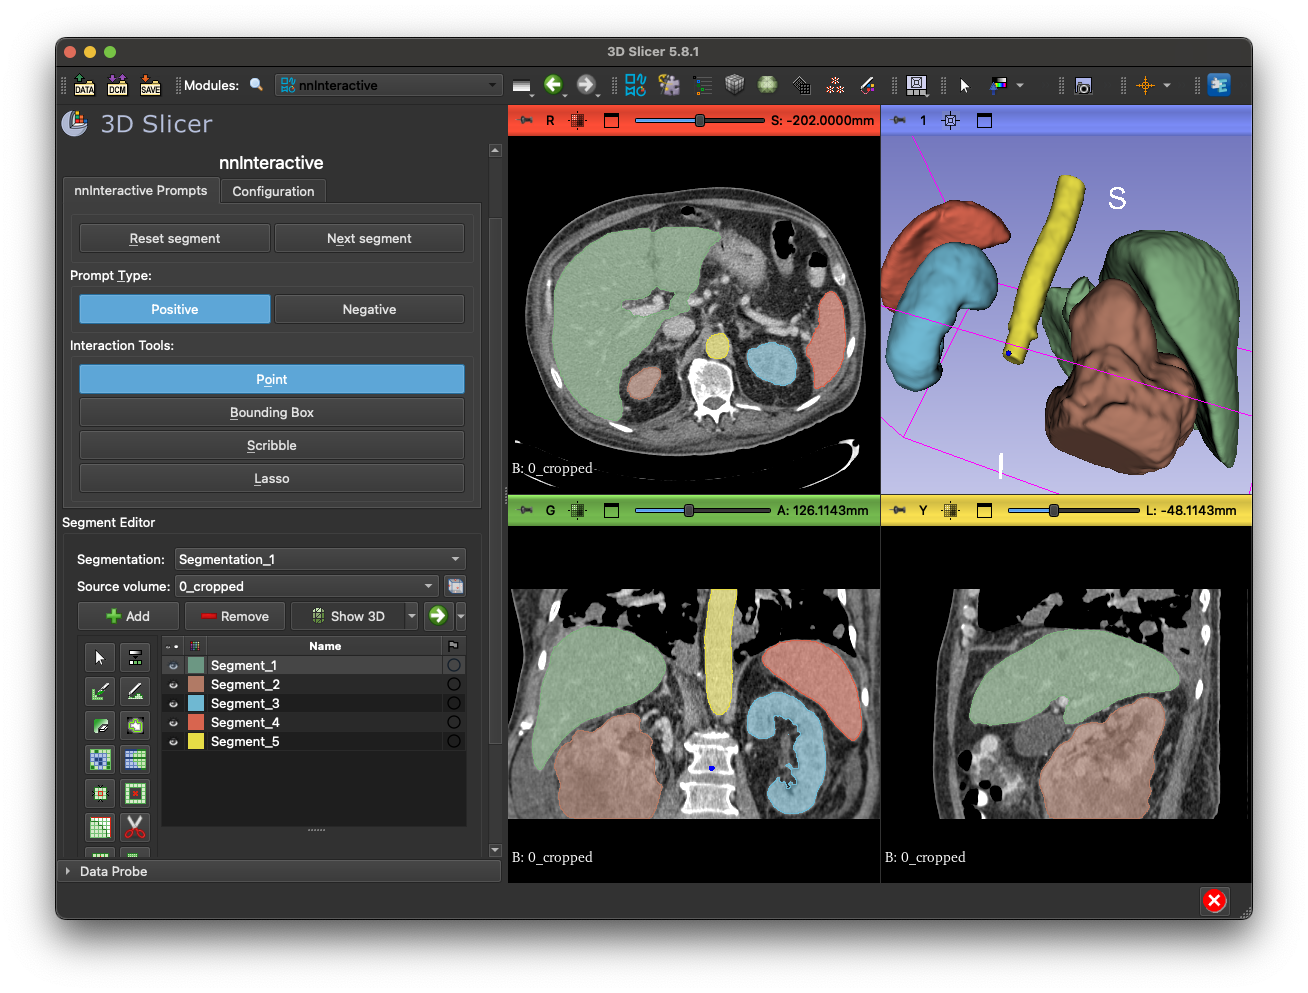
\includegraphics{img/screenshot.png}
\caption{Screenshot of the \texttt{SlicerNNInteractive}
extension.\label{fig:screenshot}}
\end{figure}

The sidebar of the user interface consists of a menu with the tabs
\emph{nnInteractive Prompts} and \emph{Configuration}, and the
\emph{Segment Editor}. The \emph{Configuration} tab allows the user to
change the Server URL. This URL is saved in \texttt{3D\ Slicer}'s
settings, which will be remembered in future sessions. The
\emph{nnInteractive Prompts} menu consists of the following sections:

\begin{itemize}
\item
  \textbf{Segment buttons:} The \emph{Reset segment} button removes all
  prompts from the current segment, and deletes the current segmentation
  on the server and client-side. The \emph{Next segment} button creates
  a new empty segment in the \emph{Segment Editor}.
\item
  \textbf{Prompt Type:} These \emph{Positive} and \emph{Negative}
  buttons manage whether the provided prompt will be interpreted as a
  positive or negative prompt, respectively.
\item
  \textbf{Interaction Tools:} The four buttons in this section activate
  or deactivate the interaction tools. When a prompt type is activated,
  the user can place the prompt in the image. When a prompt has been
  placed, the client synchronizes the image and the segment to the
  server if needed, and sends the prompt to the server. The server
  subsequently processes the prompt and sends the updated segmentation
  back. When a prompt has been placed and processed, a new prompt of the
  same type can be placed immediately.
\end{itemize}

Each button in the \emph{nnInteractive Prompts} menu has an associated
keyboard shortcut, which is indicated using the underlined letters
within the button text.

If a segment is selected in the \emph{Segment Editor}, prompts will
always be applied to that segment. Every time a user has switched
segments, the associated segmentation is uploaded to server and used as
input mask to the \texttt{nnInteractive} model. When no segment is
selected, a new segment is created automatically.

\section{Speed Measurements}\label{speed-measurements}

We measured the interaction time of \texttt{SlicerNNInteractive} for all
interaction types, in settings with lower and higher computational
resources. We automatically generated user interactions in
\texttt{3D\ Slicer}, ensuring identical prompts in all computational
settings. Each measurement was repeated 10 times, for which we report
the mean and standard deviation. The code for these automated tests is
available on
\url{https://github.com/coendevente/SlicerNNInteractive/blob/add_timing_test/slicer_plugin/SlicerNNInteractive/SlicerNNInteractive.py}.

For each interaction type, we generated automated prompts to segment the
same brain tumor in the same MRI-scan. This image was
\texttt{MRBrainTumor2} from \texttt{3D\ Slicer}'s \texttt{SampleData}
extension. We also tested interaction speed for three different image
sizes: \texttt{S}, \texttt{M}, and \texttt{L}. \texttt{L} was the
original image, with a size of 256 × 256 × 130 voxels. \texttt{M} was a
2× in each direction downsampled version of \texttt{L}, with a size of
128 × 128 × 65 voxels. \texttt{S} was a 4× in each direction downsampled
version of \texttt{L}, with a size of 64 × 64 × 32 voxels.

The client was a 14'' MacBook Pro (2021, M1 Pro, Sonoma 14.5, 16 GB
Memory, 8 CPU cores). In the lower computational resource experiments
(\texttt{L}), the server was a Linux machine with an NVIDIA GeForce GTX
1080 Ti GPU with 11 GB VRAM (Ubuntu 22.04.1, Intel® Core™ i7-6700 CPU,
48 GB RAM). In the higher computational resource experiments
(\texttt{H}), the server was a Linux machine with an NVIDIA GeForce RTX
4090 GPU with 24 GB VRAM (Ubuntu 22.04.1, 13th Gen Intel® Core™
i7-13700K CPU, 128 GB RAM).

The results of these experiments are presented in
\autoref{fig:speed_measurements}.

\begin{figure}
\centering
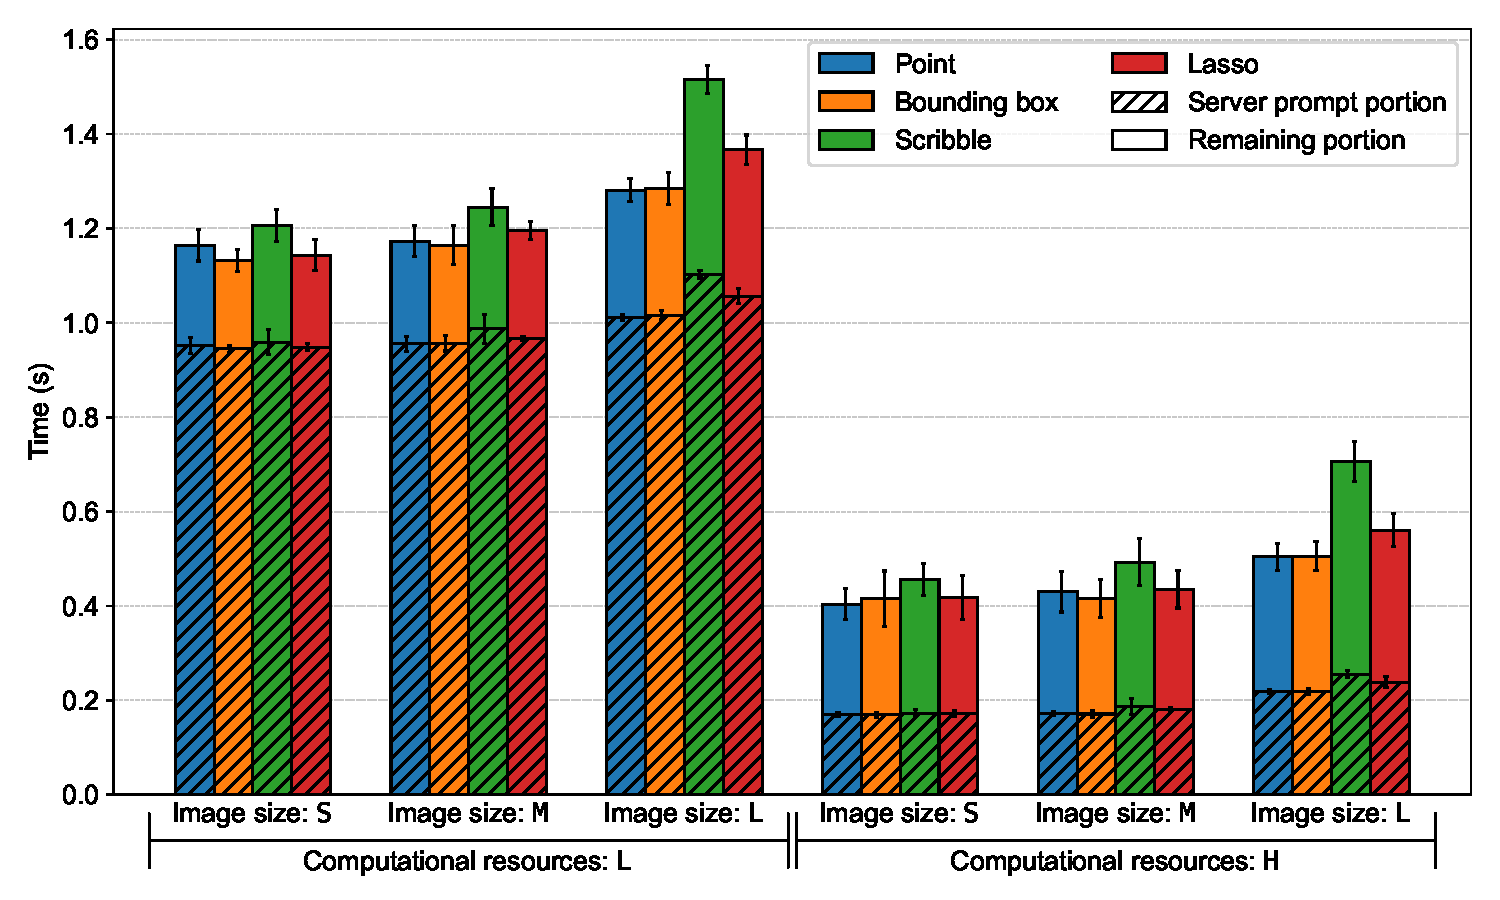
\includegraphics{img/speed_measurements.pdf}
\caption{Interaction speed measurements of \texttt{SlicerNNInteractive}.
The images with sizes \texttt{S}, \texttt{M}, and \texttt{L} were images
of small, medium, and large size, respectively. Computational resources
\texttt{L} and \texttt{H} are experiments using machines with lower and
higher computational resources, respectively. The height of each bar and
the size of each error bar represent the mean and std. dev. of 10
repeated measurements, respectively. The total height of each bar
represents the total time for an interaction to be processed by our
extension. The dashed portion of each bar represents the prompt server
request time (including model inference, prompt upload, and mask
download).\label{fig:speed_measurements}}
\end{figure}

\section{Future Work}\label{future-work}

Despite the already high interaction speed, as quantitatively measured
in this paper and noted by early users, our timing experiments show that
a large portion of the total interaction time originates from
client-side overhead -- especially for larger image sizes and better
computational resources. This overhead is due to processes such as
updating the visualized segmentation and checking for input changes.
Future work may focus on reducing this overhead to further improve
responsiveness.

Currently, the server does not support multiple clients at the same
time. \texttt{nnInteractive} releases most used VRAM instantly after
having processed a prompt, so simultaneously running multiple servers --
one for each individual user -- on one GPU is currently a viable
solution in most settings. However, in future work, we would like to
implement multi-user support through one server instance to further
improve resource efficiency.

Furthermore, for users with a sufficiently powerful local GPU, future
versions of the plugin may support local inference directly within the
Python environment of \texttt{3D\ Slicer}. With the upcoming release of
Python 3.12 in \texttt{3D\ Slicer}, this functionality will become
technically feasible. This would reduce the number of required
installation steps even further for this group of users.

\section*{References}\label{references}
\addcontentsline{toc}{section}{References}

\phantomsection\label{refs}
\begin{CSLReferences}{1}{0}
\bibitem[\citeproctext]{ref-du2024segvol}
Du, Y., Bai, F., Huang, T., \& Zhao, B. (2024). {SegVol}: Universal and
interactive volumetric medical image segmentation. \emph{Advances in
Neural Information Processing Systems}, \emph{37}, 110746--110783.

\bibitem[\citeproctext]{ref-isensee2021nnu}
Isensee, F., Jaeger, P. F., Kohl, S. A., Petersen, J., \& Maier-Hein, K.
H. (2021). {nnU-Net}: A self-configuring method for deep learning-based
biomedical image segmentation. \emph{Nature Methods}, \emph{18}(2),
203--211. \url{https://doi.org/10.1038/s41592-020-01008-z}

\bibitem[\citeproctext]{ref-isensee2025nninteractive}
Isensee, F., Rokuss, M., Krämer, L., Dinkelacker, S., Ravindran, A.,
Stritzke, F., Hamm, B., Wald, T., Langenberg, M., Ulrich, C., Deissler,
J., Floca, R., \& Maier-Hein, K. (2025). nnInteractive: Redefining 3D
promptable segmentation. \emph{arXiv Preprint arXiv:2503.08373}.
\url{https://doi.org/10.48550/arXiv.2503.08373}

\bibitem[\citeproctext]{ref-isensee2024nnu}
Isensee, F., Wald, T., Ulrich, C., Baumgartner, M., Roy, S., Maier-Hein,
K., \& Jaeger, P. F. (2024). {nnU-Net} revisited: A call for rigorous
validation in {3D} medical image segmentation. \emph{International
Conference on Medical Image Computing and Computer-Assisted
Intervention}, 488--498. \url{https://doi.org/10.48550/arXiv.2404.09556}

\bibitem[\citeproctext]{ref-Kikinis2014}
Kikinis, R., Pieper, S. D., \& Vosburgh, K. G. (2014). 3D slicer: A
platform for subject-specific image analysis, visualization, and
clinical support. In F. A. Jolesz (Ed.), \emph{Intraoperative imaging
and image-guided therapy} (pp. 277--289). Springer New York.
\url{https://doi.org/10.1007/978-1-4614-7657-3_19}

\bibitem[\citeproctext]{ref-kirillov2023segment}
Kirillov, A., Mintun, E., Ravi, N., Mao, H., Rolland, C., Gustafson, L.,
Xiao, T., Whitehead, S., Berg, A. C., Lo, W.-Y., Dollar, P., \&
Girshick, R. (2023). Segment anything. \emph{Proceedings of the IEEE/CVF
International Conference on Computer Vision}, 4015--4026.

\bibitem[\citeproctext]{ref-MITK_Team_MITK_2024}
MITK~Team. (2024). \emph{{MITK}} (Version v2024.12).
\url{https://github.com/MITK/MITK}

\bibitem[\citeproctext]{ref-ravi2024sam}
Ravi, N., Gabeur, V., Hu, Y.-T., Hu, R., Ryali, C., Ma, T., Khedr, H.,
Rädle, R., Rolland, C., Gustafson, L., Mintun, E., Pan, J., Alwala, K.
V., Carion, N., Wu, C.-Y., Girshick, R., Dollár, P., \& Feichtenhofer,
C. (2024). {SAM} 2: Segment anything in images and videos. \emph{arXiv
Preprint arXiv:2408.00714}.
\url{https://doi.org/10.48550/arXiv.2408.00714}

\bibitem[\citeproctext]{ref-Sofroniew2025-ty}
Sofroniew, N., Lambert, T., Bokota, G., Nunez-Iglesias, J., Sobolewski,
P., Sweet, A., Gaifas, L., Evans, K., Burt, A., Doncila Pop, D.,
Yamauchi, K., Weber Mendonça, M., Buckley, G., Vierdag, W.-M., Royer,
L., Can Solak, A., Harrington, K. I. S., Ahlers, J., Althviz Moré, D.,
\ldots{} Zhao, R. (2025). \emph{Napari: A multi-dimensional image viewer
for python}. Zenodo. \url{https://doi.org/10.5281/zenodo.8115575}

\bibitem[\citeproctext]{ref-wang2023sam}
Wang, H., Guo, S., Ye, J., Deng, Z., Cheng, J., Li, T., Chen, J., Su,
Y., Huang, Z., Shen, Y., \& others. (2023). {SAM-Med3D}: Towards
general-purpose segmentation models for volumetric medical images.
\emph{arXiv Preprint arXiv:2310.15161}.
\url{https://doi.org/arXiv.2310.15161}

\end{CSLReferences}

\end{document}
